%!TeX root=../tese.tex
%("dica" para o editor de texto: este arquivo é parte de um documento maior)
% para saber mais: https://tex.stackexchange.com/q/78101/183146

%% ------------------------------------------------------------------------- %%
\chapter{Interpretação geométrica de buscas em ABBs}
\label{cap:geometria}

Neste capítulo explicaremos o que são conjuntos de pontos arboreamente independente e como interpretar de maneira geométrica algoritmos de busca em ABBs.

\section{Conjuntos arboreamente satisfeitos}

Chamamos dois pontos $a$ e $b$ de \textit{ortogonalmente colineares} se $a$ e $b$ estão na mesma linha horizontal ou vertical. Se $a$ e $b$ não são ortogonalmente colineares, denotamos por \textit{$\{a,b\}$-retângulo} o retângulo ortogonal que tem $a$ e $b$ como vértices.

Um par de pontos $\{a,b\}$ de um conjunto de pontos $P$ é \textit{arboreamente satisfeito} se $a$ e $b$ são ortogonalmente colineares ou se há pelo menos um ponto do conjunto \( P \setminus \{a,b\} \) que está dentro da região delimitada pelo \{a,b\}-retângulo, incluindo seu perímetro. Um conjunto $P$ de pontos é \textit{arboreamente satisfeito} se todos os pares de pontos do conjunto são arboreamente satisfeitos. Veja a Figura~\ref{fig:geometria-inicial}.

\begin{figure}[h!]
    \centering
    \begin{minipage}[b]{0.45\textwidth}
        \centering
        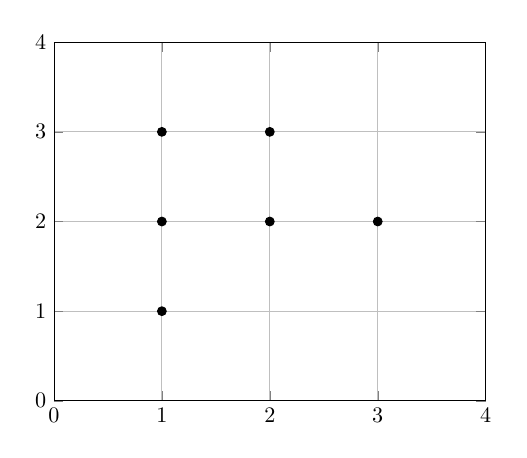
\begin{tikzpicture}[scale=0.8]
        \begin{axis}[
            grid=major,
            xmin=0, xmax=4,
            ymin=0, ymax=4,
            xtick={0,1,2,3,4},
            ytick={0,1,2,3,4}
        ]
        \addplot[only marks, mark=*] coordinates {
            (1,1)
            (1,2)
            (1,3)
            (2,2)
            (2,3)
            (3,2)
        };
        \end{axis}
        \end{tikzpicture}
    \end{minipage}\hfill
    \begin{minipage}[b]{0.45\textwidth}
        \centering
        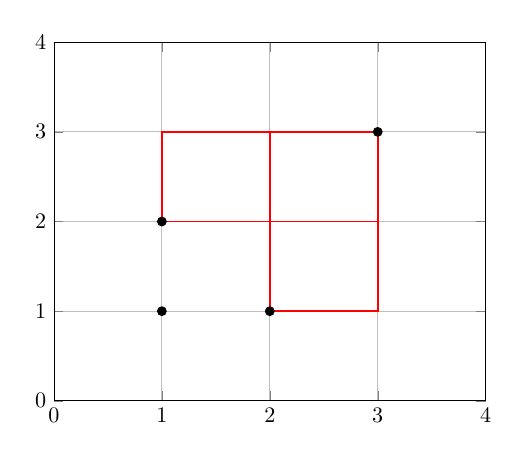
\begin{tikzpicture}[scale=0.8]
        \begin{axis}[
            grid=major,
            xmin=0, xmax=4,
            ymin=0, ymax=4,
            xtick={0,1,2,3,4},
            ytick={0,1,2,3,4}
        ]
        \addplot[only marks, mark=*] coordinates {
            (1,1)
            (1,2)
            (2,1)
            (3,3)
        };
        \addplot[
            color=red,
            line width=0.7pt
        ]
        coordinates {
            (2,1)
            (3,1)
            (3,3)
            (2,3)
            (2,1)
        };
        \addplot[
            color=red,
            line width=0.7pt
        ]
        coordinates {
            (1,2)
            (3,2)
            (3,3)
            (1,3)
            (1,2)
        };
        \end{axis}
        \end{tikzpicture}
    \end{minipage}
    \caption{À esquerda, um conjunto $P$ de pontos arboreamente satisfeito. À direita, um conjunto $P$ de pontos com dois pares de pontos arboreamente insatisfeitos com seus retângulos destacados.}
\label{fig:geometria-inicial}
\end{figure}

\begin{lemma}
\label{lem:pontos_em_arestas_incidentes}
Em um conjunto arboreamente satisfeito $P$, para todo par de pontos $\{a,b\}$ não ortogonalmente colineares, há sempre pelo menos um ponto de \( P \setminus \{a,b\} \) que está em um dos lados do $\{a,b\}$-retângulo que incide em $a$, e há sempre também pelo menos um ponto de \( P \setminus \{a,b\} \) que está em um dos lados do $\{a,b\}$-retângulo que incide em $b$.
\end{lemma}


\begin{figure}
    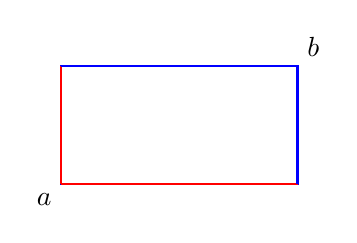
\begin{tikzpicture}[scale=1.5]
        \draw[blue, thick] (0,0) rectangle (2,1);
        
        \node at (0,0) [below left] {$a$};
        \node at (2,1) [above right] {$b$};
        
        \draw[red, thick] (0,0) -- (0,1);
        \draw[red, thick] (0,0) -- (2,0);
        \draw[blue, thick] (2,1) -- (0,1);
        \draw[blue, thick] (2,1) -- (2,0);
    \end{tikzpicture}
    \caption{O $\{a,b\}$-retângulo. Em vermelho estão destacados os lados do retângulo que incidem em $a$ e em azul estão destacados os lados que incidem em $b$.}
\end{figure}

\begin{proof} Sejam $a$ e $b$ dois pontos não ortogonalmente colineares de um conjunto arboreamente satisfeito $P$. Como $\{a,b\}$ é um par de pontos arboreamente satisfeito não ortogonalmente colineares, então a região delimitada pelo $\{a,b\}$-retângulo possui pelo menos um ponto de $P$ diferente de $\{a,b\}$. Denotemos por $c$ tal ponto. Se $c$ não estiver em um lado do $\{a,b\}$-retângulo que incide em $a$, então $a$ e $c$ não são ortogonalmente colineares e o $\{a,c\}$-retângulo está contido no $\{a,b\}$-retângulo, logo é também arboreamente satisfeito e é possível recursivamente procurar tal ponto no $\{a,c\}$-retângulo. Analogamente, se $c$ não estiver em um lado do $\{a,b\}$-retângulo que incide em $b$, então é possível recursivamente procurar tal ponto no $\{b,c\}$-retângulo, que também é arboreamente satisfeito.
\end{proof}

%Seja $\tau_i$ a subárvore // falar de subarvores?

\section{Visão geométrica de buscas}

No modelo de computação adotado, para realizar um acesso em uma ABB, o algoritmo de busca inicia o nó corrente na raiz da ABB. Em seguida, percorre a árvore descendo para o filho apropriado por meio de comparações até alcançar a chave procurada.

Dada uma sequência $X = (x_{1},\ldots,x_{m})$ de $m$ acessos às chaves $1,2,\ldots,n$, é possível ilustrar essa sequência $X$ de maneira gráfica em um plano cartesiano da seguinte forma: o eixo $x$ representará as chaves armazenadas na ABB e o eixo $y$ representará os índices $i = 1,2,\ldots,m$, que interpretamos como o tempo. Assim, um ponto de coordenada ($x$,$i$) representa a busca da chave $x$ na ABB no instante de tempo $i$, ou seja, representa $x_i$. Veja o exemplo da Figura~\ref{fig:busca_padrao}.

\begin{figure}
    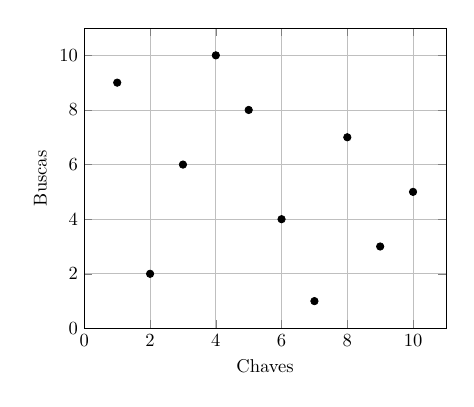
\begin{tikzpicture}[scale=0.67]
        \begin{axis}[
            xlabel={Chaves},
            ylabel={Buscas},
            grid=major,
            xmin=0, xmax=11,
            ymin=0, ymax=11,
            xtick={0,2,4,6,8,10},
            ytick={0,2,4,6,8,10}
        ]
        \addplot[only marks, mark=*] coordinates {
            (1,9)
            (2,2)
            (3,6)
            (4,10)
            (5,8)
            (6,4)
            (7,1)
            (8,7)
            (9,3)
            (10,5)
        };
        \end{axis}
    \end{tikzpicture}
    \caption{Gráfico representando a sequência (7, 2, 9, 6, 10, 3, 8, 5, 1, 4) de acessos.}
\label{fig:busca_padrao}
\end{figure}

A \textit{visão geométrica da execução de um algoritmo de busca em ABB} para uma sequência $X = (x_{1},\ldots,x_{m})$ de buscas, de maneira similar, é o conjunto de pontos na forma ($x$,$i$) tal que $x$ foi uma das chaves visitadas durante a busca pela chave $x_i$. Para cada $i \in \{1,\ldots,m\}$, esse conjunto de pontos esta sob a reta $y = i$ e representa os nós visitados durante a busca por $x_i$. Veja a Figura~\ref{fig:traducao-busca-em-ASS}.

\begin{figure}[h!]
    \centering
    \begin{minipage}[b]{0.34\textwidth}
        \centering
        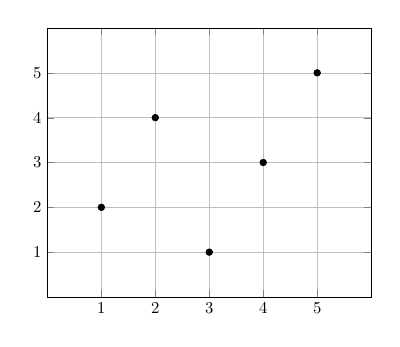
\begin{tikzpicture}[scale=0.6]
        \begin{axis}[
            grid=major,
            xmin=0, xmax=6,
            ymin=0, ymax=6,
            xtick={1,2,3,4,5},
            ytick={1,2,3,4,5}
        ]
        \addplot[only marks, mark=*] coordinates {
            (3,1)
            (1,2)
            (4,3)
            (2,4)
            (5,5)
        };
        \end{axis}
        \end{tikzpicture}
    \end{minipage}\hfill
    \begin{minipage}[b]{0.33\textwidth}
        \centering
        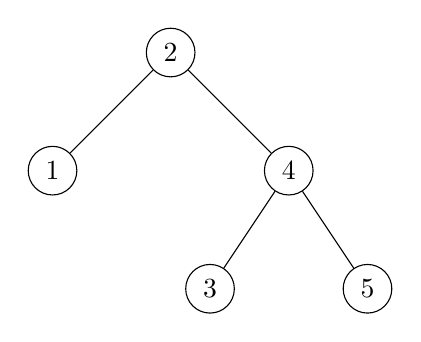
\begin{tikzpicture}
            [node/.style={circle,draw,minimum size=1.5em}]
            \node[node] (A) at (-1.5,-1.5) {$1$};
            \node[node] (B) at (0,0) {$2$};
            \node[node] (C) at (0.5,-3) {$3$};
            \node[node] (D) at (1.5,-1.5) {$4$};
            \node[node] (E) at (2.5,-3) {$5$};
            
            \draw (A) -- (B);
            \draw (B) -- (D);
            \draw (C) -- (D);
            \draw (E) -- (D);
          \end{tikzpicture}
    \end{minipage}\hfill
    \begin{minipage}[b]{0.33\textwidth}
        \centering
        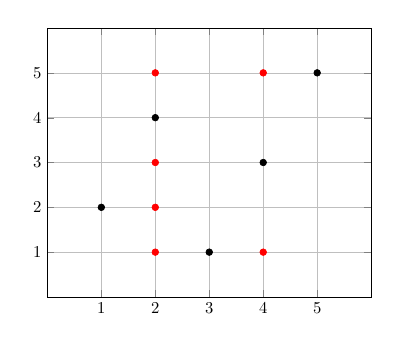
\begin{tikzpicture}[scale=0.6]
            \begin{axis}[
                grid=major,
                xmin=0, xmax=6,
                ymin=0, ymax=6,
                xtick={1,2,3,4,5},
                ytick={1,2,3,4,5}
            ]
            \addplot[only marks, mark=*] coordinates {
                (3,1)
                (1,2)
                (4,3)
                (2,4)
                (5,5)
            };
            \addplot[color=red, only marks, mark=*] coordinates {
                (2,1)
                (4,1)
                (2,2)
                (2,3)
                (2,5)
                (4,5)
            };
            \end{axis}
            \end{tikzpicture}
    \end{minipage}
    \caption{À esquerda, o conjunto de pontos que representa a sequência $X = (3,1,4,2,5)$. No meio, uma possível ABB com as chaves \{1,2,\ldots,5\}. À direita, o conjunto correspondente aos nós da ABB ao centro, visitados pelo algoritmo de busca que não efetua rotações, os pontos pretos são os nós da sequência $X$ de acessos e os pontos vermelhos são o restante dos nós visitados durante cada um desses acessos. Note que o conjunto de pontos à esquerda não é arboreamente satisfeito, mas o conjunto à direita é.}
\label{fig:traducao-busca-em-ASS}
\end{figure}

\begin{lemma} A visão geométrica de qualquer execução de um algoritmo de busca em ABB no modelo de computação adotado é um conjunto de pontos arboreamente satisfeitos.
\label{lema:visao_geometrica_vira_ASS}
\end{lemma}

\begin{proof}
Assuma que a visão geométrica de um algoritmo de busca em uma ABB $T$ não é arboreamente satisfeita. Dessa maneira, há pelo menos um par $\{a,b\}$ de pontos nesse conjunto que não é arboreamente satisfeito. Seja $i$ o instante de tempo que a chave $a$ foi visitada, e seja $j$ o instante de tempo que a chave $b$ foi visitada. Assumiremos também sem perda de generalidade que $i < j$ e $a < b$.

Seja $c$ o ancestral comum mais profundo de $a$ e $b$ em $T$ imediatamente antes da busca $i$. E seja $d$ o ancestral comum mais profundo de $a$ e $b$ em $T$ imediatamente antes da busca $j$.

Os quatro lados do $\{a,b\}$-retângulo terão um papel a seguir na prova. Eles são\\
$\ell_1$ = \{$(x,y)$ | $x = a$ e $i < y \leq j$\}, representando todas as visitas a chave $a$ entre os instantes de tempo $i$ e $j$. \\
$\ell_2$ = \{$(x,y)$ | $a \leq x < b$ e $y = j$\}, representando todas as visitas a chaves entre $a$ e $b$ no instante de tempo $j$. \\
$\ell_3$ = \{$(x,y)$ | $x = b$ e $i \leq y < j$\}, representando todas as visitas a chave $b$ entre os instantes de tempo $i$ e $j$. \\
$\ell_4$ = \{$(x,y)$ | $a < x \leq b$ e $y = i$\}, representando todas as visitas a chaves entre $a$ e $b$ no instante de tempo $i$. \\

Como $\{a,b\}$ é um par de pontos arboreamente insatisfeitos, nota-se que não há nenhum ponto tanto nas bordas quanto no interior do $\{a,b\}$-retângulo. Logo, $\ell_1 \cup \ell_2 \cup \ell_3 \cup \ell_4 = \emptyset$.

Vale ressaltar que se $e$ é o ancestral comum mais profundo de $a$ e $b$ em $T$, então sabemos que $a \leq e \leq b$ e, mais importante, $e$ está mais acima em $T$ em comparação com $a$ e $b$ (possivelmente na mesma profundidade caso seja igual a $a$ ou $b$). Assim, $e$ está no caminho da raiz da ABB até qualquer chave no intervalo $[a,b]$. Em outras palavras, para visitar qualquer chave no intervalo $[a,b]$, é necessário visitar o ancestral comum mais profundo entre $a$ e $b$.

\begin{figure}[H]
    \centering
    \vfill % Adiciona espaço acima da figura para centralização vertical
    \begin{minipage}[t]{0.6\textwidth}
        Se $\ell_2 = \emptyset$, então obrigatoriamente $d = b$. Se $c = b$, então $\ell_3 \neq \emptyset$. Se $c \neq b$, então em pelo menos algum outro instante de tempo $h$, $h < j$, $b$ teve que ser visitado para ser rotacionado até virar o ancestral comum mais profundo entre $a$ e $b$, logo $\ell_3 \neq \emptyset$.   

        Se $\ell_4 = \emptyset$, então $c = a$. Porém, no instante $j$, $b$ é acessado. Caso $c = d = a$, $a$ precisa ser visitado no instante de tempo $j$, logo $\ell_1 \neq \emptyset$. Caso $c \neq d$, então em algum instante de tempo $h$, $i \leq h < j$, o ancestral comum mais profundo entre $a$ e $b$ mudou, logo algum nó com chave no intervalo $(a,b]$ precisa ter sido rotacionado para cima, porém sabemos que para visitar qualquer chave no intervalo $[a,b]$ no instante de tempo $h$, é necessário visitar o ancestral comum mais profundo que neste caso é $a$. Logo $\ell_1 \neq \emptyset$. 
    \end{minipage}\hfill
    \begin{minipage}[t]{0.4\textwidth}
        % Coluna da direita com a imagem e a legenda
        \centering
        \begin{figure}[H]
            \centering
            \begin{adjustbox}{valign=t, raise=-25pt} % Alinha o gráfico ao topo da caixa
            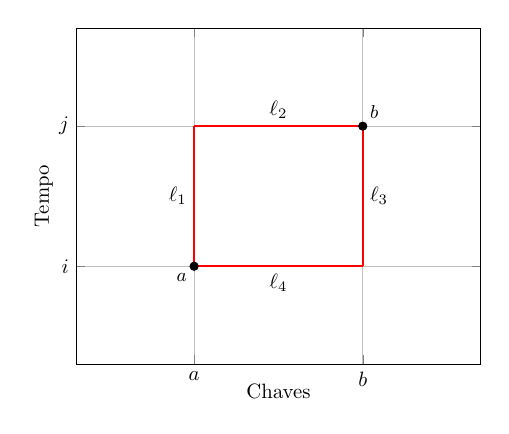
\begin{tikzpicture}[scale=0.75]
            \begin{axis}[
                xlabel={Chaves},
                ylabel={Tempo},
                grid=major,
                xmin=0.3, xmax=2.7,
                ymin=0.3, ymax=2.7,
                xtick={1,2},
                ytick={1,2},
                xlabel style={at={(axis description cs:0.5,-0.08)}, anchor=center}, % Ajusta a posição do rótulo do eixo x
                ylabel style={at={(axis description cs:-0.08,0.5)}, anchor=center},
                xticklabels={$a$,$b$}, % Define os rótulos do eixo x
                yticklabels={$i$,$j$} % Define os rótulos do eixo y
            ]

            \addplot[only marks, mark=*] coordinates {
                (1,1)
                (2,2)
            };

            \addplot[red, thick] coordinates {
                (1,2)
                (2,2)
            };

            \addplot[red, thick] coordinates {
                (2,2)
                (2,1)
            };

            \addplot[red, thick] coordinates {
                (1,1)
                (1,2)
            };

            \addplot[red, thick] coordinates {
                (1,1)
                (2,1)
            };

            % Adiciona rótulos aos pontos
            \node at (axis cs:1,1) [anchor=north east, fill=white, font=\small] {$a$};
            \node at (axis cs:2,2) [anchor=south west, fill=white, font=\small] {$b$};

            \node at (axis cs:1,1.5) [anchor=east, font=\normalsize] {$\ell_1$};
            \node at (axis cs:1.5,2) [anchor=south, font=\normalsize] {$\ell_2$};
            \node at (axis cs:2,1.5) [anchor=west, font=\normalsize] {$\ell_3$};
            \node at (axis cs:1.5,1) [anchor=north, font=\normalsize] {$\ell_4$};
            %\node at (axis cs:1.5,1.5) [anchor=center, font=\normalsize] {5};

            \end{axis}
            \end{tikzpicture}
            \end{adjustbox}
            \label{fig:tikz-captions}
        \end{figure}
    \end{minipage}
    \vfill % Adiciona espaço abaixo da figura para centralização vertical
    \label{fig:chaves-buscas}
\end{figure}

Por contra-positiva das conclusões acima, temos:
\begin{center}
Se $\ell_3 = \emptyset \Rightarrow \ell_2 \neq \emptyset$. \\
Se $\ell_1 = \emptyset \Rightarrow \ell_4 \neq \emptyset$.
\end{center}

Conclui-se então que $\ell_1 \cup \ell_4  \neq \emptyset$ e $\ell_2 \cup \ell_3  \neq \emptyset$, e assim chegamos numa contradição.

Vale ressaltar que é conveniente que $\ell_1 \cup \ell_4  \neq \emptyset$ e $\ell_2 \cup \ell_3  \neq \emptyset$, uma vez que $\ell_1 \cup \ell_4$ representa os pontos pertencentes ao $\{a,b\}$-retângulo incidentes ao vértice $a$ e  $\ell_2 \cup \ell_3$ representa os pontos pertencentes ao $\{a,b\}$-retângulo incidentes ao vértice $b$. Assim, respeitando o Lema~\ref{lem:pontos_em_arestas_incidentes}.
\end{proof}

\begin{lemma}Qualquer conjunto de pontos arboreamente satisfeito representa a execução de um algoritmo de busca em ABB no modelo de computação adotado.
\end{lemma}

\begin{proof}

É possível criar uma treap com nós que possuem a coordenada $x$ como chave. Usaremos o campo prioridade dos nós da treap para representar o próximo instante de tempo que tal chave é visitada. Seja $N(x,i)$ a próximo visita à chave $x$ depois do instante de tempo $i$, ou seja, o ponto ($x$,p.y) do conjunto com menor p.y > $i$. Se não há mais visitas a chave $x$ depois do tempo $i$, ou seja, não há nenhum ponto no conjunto com coordenadas ($x$,p.y) com p.y > $i$, então definimos $N(x,i) = \infty$. Os nós (chave, prioridade) da treap são inicializadas como ($x$, $N(x,0)$) e no instante de tempo $t$ as chaves estão no formato ($x$, $N(x,t)$).

No instante de tempo $i$, os nós visitados, ou seja, todos os pontos do conjunto arboreamente satisfeito com coordenada $y=i$, formam uma subárvore que possui a raiz. Para reorganizar os nós de maneira a manter a propriedade heap da prioridade da treap para o instante de tempo $i+1$, é preciso reconfigurar os nós visitados de maneira a manter os nós que serão visitados mais , mais superficiais e os nós que serão visitados mais tarde, mais profundos. Na prática, basta manter a prioridade de heap mínimo da treap em relação ao $N(x,i)$.

Se conseguirmos manter a estrutura da treap após cada busca apenas visitando os elementos dados pelo conjunto arboreamente satisfeito, então descrevemos um algoritmo offline que visita todos os elementos da sequência de entrada e evidentemente traduz um conjunto arboreamente satisfeito em um algoritmo de busca em ABB.

Vamos supor por contradição que não é possível manter a estrutura da treap entre o instante de tempo $i$ e $i+1$. Se não é possível manter tal estrutura, isso significa que há duas chaves, nomeadas $a$ e $b$ ($a \neq b$), tal que $a$ está contida na subárvore das chaves visitas no instante de tempo $i$ e $b$ não é visitada no instante de tempo $i$ e não consegue ser visitada no instante de tempo $i+1$ apenas com os pontos do conjunto arboreamente satisfeito. Assim, $N(a,i) > N(b,i)$. Assumiremos sem perda de generalidade que $a < b$ e o nó de $b$ é filho do nó de $a$ na ABB durante o instante de tempo $i$. Veja a Figura~\ref{fig:representacao_grafica}.

De maneira informal, $a$ é uma chave que foi visitada no tempo $i$ e $b$ é filha de $a$ e não foi visitada no tempo $i$. O próximo acesso de $b$ é mais cedo que o próximo acesso de $a$. Para contradizer o lema, precisamos provar que um conjunto ser arboreamente satisfeito não é condição suficiente para garantir a manutenção da estrutura da treap de maneira adequada entre quaisquer instantes de tempo.

\begin{figure}
    \begin{tikzpicture}
        \coordinate (A) at (0, 0);
        \coordinate (B) at (3, 0);
        \coordinate (C) at (1.5, 2.6);
    
        \draw (A) -- (B) -- (C) -- cycle;
    
        \path (A) ++(0,1) coordinate (start);
        \path (start) ++(3,0.7) coordinate (end);
        \draw[dashed] (start) -- (end) node[midway,below] {};
    
        \path (start) ++(1.5,0.57) coordinate (x);
        \path (start) ++(1.7,0.2) coordinate (y);

        \begin{scope}
            \clip (A) -- (B) -- (C) -- cycle; % Clipping para definir a área do triângulo
            \fill[pattern=vertical lines] (A) -- (C) -- (end) -- (start) -- cycle; % Preenchimento hachurado
        \end{scope}
    
        %\filldraw (x) circle (2pt) node[anchor=south] {};
        %\filldraw (y) circle (2pt) node[anchor=north] {};
    
        \draw[red, thick] (x) -- (y);

        \filldraw (x) circle (1.5pt) node[anchor=south] {a};
        \filldraw (y) circle (1.5pt) node[anchor=north] {b};

        \draw[->, black] (1.8,1.8) -- (2.5,2) node[pos=1, right] {Chaves visitadas no instante de tempo $i$};
    \end{tikzpicture}
    \caption{Representação da situação descrita. Simplificação do formato de uma ABB por um triângulo, a área destacada representa todos os nós acessados no instante de tempo $i$. A chave $b$ não foi visitada nesse instante de tempo.}
\label{fig:representacao_grafica}
\end{figure}

Os lados a seguir terão um papel na prova e estão representados na Figura~\ref{fig:area_delimitada}. \\
$\ell_1$ = \{$(x,y)$ | $x = a$ e $i < y \leq i+1$\}, representando todas as visitas a chave $a$ entre os instantes de tempo $i$ e $i+1$. \\
$\ell_2$ = \{$(x,y)$ | $a < x \leq b$ e $y = i$\}, representando todas as visitas a chaves entre $a$ e $b$ no instante de tempo $i$. \\


\begin{figure}[H]
    \centering
    \begin{adjustbox}{valign=t, raise=-25pt} % Alinha o gráfico ao topo da caixa
    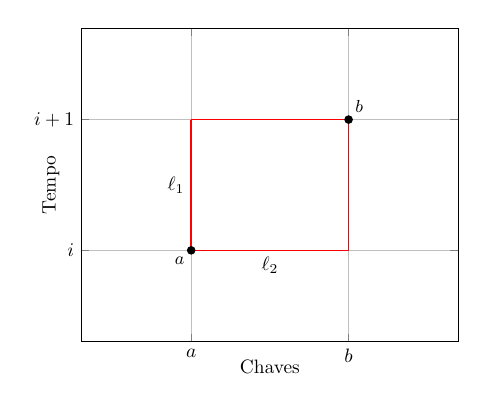
\begin{tikzpicture}[scale=0.7]
    \begin{axis}[
        xlabel={Chaves},
        ylabel={Tempo},
        grid=major,
        xmin=0.3, xmax=2.7,
        ymin=0.3, ymax=2.7,
        xtick={1,2},
        ytick={1,2},
        xlabel style={at={(axis description cs:0.5,-0.08)}, anchor=center}, % Ajusta a posição do rótulo do eixo x
        ylabel style={at={(axis description cs:-0.08,0.5)}, anchor=center},
        xticklabels={$a$,$b$}, % Define os rótulos do eixo x
        yticklabels={$i$,$i+1$} % Define os rótulos do eixo y
    ]

    \addplot[only marks, mark=*] coordinates {
        (1,1)
        (2,2)
    };

    \addplot[red, thick] coordinates {
        (1,2)
        (2,2)
    };

    \addplot[red, thick] coordinates {
        (2,2)
        (2,1)
    };

    \addplot[red, thick] coordinates {
        (1,1)
        (1,2)
    };

    \addplot[red, thick] coordinates {
        (1,1)
        (2,1)
    };

    % Adiciona rótulos aos pontos
    \node at (axis cs:1,1) [anchor=north east, fill=white, font=\small] {$a$};
    \node at (axis cs:2,2) [anchor=south west, fill=white, font=\small] {$b$};

    \node at (axis cs:1,1.5) [anchor=east, font=\normalsize] {$\ell_1$};
    \node at (axis cs:1.5,1) [anchor=north, font=\normalsize] {$\ell_2$};

    \end{axis}
    \end{tikzpicture}
    \end{adjustbox}
    \caption{$\{a,b\}$-retângulo.}
\label{fig:area_delimitada}
\end{figure}

De acordo com o Lema~\ref{lem:pontos_em_arestas_incidentes}, como $\{a,b\}$ representa um par de pontos arboreamente satisfeitos, então há pelo menos um outro ponto em alguma das arestas do $\{a,b\}$-retângulo que incide em $a$. Como $N(a,i) > N(b,i)$, então sabemos que a área $\ell_1$ não possui pontos no conjunto arboreamente satisfeito. Logo, para o Lema~\ref{lem:pontos_em_arestas_incidentes} ser verdadeiro, alguma chave entre $a$ e $b$ deve ter sido visitada no instante de tempo $i$, ou seja, $\ell_2 \neq \emptyset$. 

Como $b$ é filho direito de $a$, então para acessar qualquer chave no intervalo ($a,b$) no instante de tempo $i$, pela propriedade de ordenação de ABBs, é necessário acessar a chave $b$, pois as chaves neste intervalo são mais profundas que $a$ e $b$. 

Assim, para o par de pontos $\{a,b\}$ ser arboreamente satisfeito é preciso que alguma chave no intervalo ($a,b$) tenha sido visitada no instante de tempo $i$, porém para acessar alguma destas chave neste instante de tempo é preciso acessar a chave $b$, e a suposição inicial era que $b$ não era visitada neste instante de tempo. Chegamos numa contradição.

Assim, nota-se que a reestruturação da treap da maneira proposta é sempre válida em conjuntos de pontos arboreamente satisfeitos e tal reestruturação é um algoritmo offline que converte um conjunto de pontos arboreamente satisfeitos em uma execução de um algoritmo de busca em ABB.
\end{proof}

